\documentclass[12pt]{article}

\usepackage[spanish, es-tabla, es-nodecimaldot]{babel}
\usepackage[utf8x]{inputenc}
\usepackage{amsmath}

\usepackage{hyperref}
\usepackage{url}
\usepackage{textcomp}
\usepackage{gensymb}
\usepackage[dvipsnames]{xcolor}

\usepackage{parskip}
\usepackage{fancyhdr}
\usepackage{multicol}
\usepackage{vmargin}
\usepackage{setspace}
\usepackage{geometry}

\usepackage{float}
\usepackage{array}
\usepackage{graphicx}
\graphicspath{{images/}}
\usepackage{wrapfig}
\usepackage{caption}
\usepackage{subcaption}

\setmarginsrb{2 cm}{1 cm}{2 cm}{1.5 cm}{0.5 cm}{1 cm}{1 cm}{1 cm} %{izq}{up}{der}{down}{Encabezado}
\title{Radiación}
\author{Martín Alejandro Paredes Sosa}		

\makeatletter
\let\thetitle\@title
\let\theauthor\@author
\let\thedate\@date										
\makeatother

\pagestyle{fancy}
\fancyhf{}
%\rhead{Lic.. Física}
%\lhead{Informe 5: \thetitle}
\cfoot{\thepage}

\begin{document}
%====================================================================
\begin{center}
{ \large \bfseries \thetitle}
\end{center}
	\begin{minipage}{\textwidth}
		\begin{center} 
			\theauthor 
			\end{center}
	\end{minipage}
%===================================================================================================
\begin{abstract}
En esta experiencia se realizaron dos actividades cuyo principal objetivo era determinar el comportamiento de la radiación infrarroja y la temperatura de distintos materiales.
\end{abstract}
\vspace{-1cm}
%===================================================================================================
\section{Introducción}
\vspace{-0.5cm}
La radiación a la transmisión de calor entre dos cuerpos los cuales, en un instante dado, tienen temperaturas distintas, sin que entre ellos exista contacto ni conexión por otro sólido conductor. Es una forma de emisión de ondas electromagnéticas (asociaciones de campos eléctricos y magnéticos que se propagan a la velocidad de la luz) que emana todo cuerpo que esté a mayor temperatura que el cero absoluto. 

Esta experiencia se divide en dos:
Para la primera actividad se utiliza un cubo llamado "cavidad térmica", está construido de aluminio y presenta externamente diferentes tipos de superficies en sus 4 caras laterales. Este cubo es alimentado por un amplificador de potencia con una condición fija de 10 V, esto par mantener la temperatura de las paredes del cubo.

En la segunda actividad se determinará la temperatura de un filamento de tungsteno de la lámpara llamada Stefan-Boltzmann. Dicha temperatura puede ser determinada a tráves de la siguiente relación:

\begin{equation}
T = \frac{R- R_{ref}}{aR_{ref}} + T_{ref}
\end{equation}


donde
\begin{itemize}
\item R es la resistencia a la temperatura T
\item $R_{ref}$ es la resistencia a la temperatura $T_{ref}$
\item $\alpha$ es el coeficiente de resistividad del filamento ($\alpha = 4.5 x 10^{-3}$)
\end{itemize}


\vspace{-0.5cm}
%===================================================================================================
\section{Desarrollo Experimental}
\vspace{-0.5cm}
El desarrollo se divide en las dos actividades, comenzando con la de cavidad térmica.

Para esta actividad, se cuantificó la emisión de radiación usando un sensor de infrarrojo y para la temperatura se colocó un termistor, ambos conectados a la interfaz DataStudio para observar los resultados.

El sensor de radiación se colocó sobre el centro de una cara del cubo aproximadamente a 2 cm de distancia y antes de comenzar a tomar mediciones se colocó un material aislante entre el cubo y el sensor para evitar que el sensor se calentara.

Para la segunda actividad, primero se midió la resistencia a temperatura ambiente del filamento, en el caso de la lámpara el fabricante proporciona el valor de $0.84 \Omega$.
Después se alimentó la lámpara con un amplificador de potencia con un valor fijo de voltaje de 10 V.


%===================================================================================================

\section{Resultados}
Los resultados también se dividen por actividad.

Para la primer actividad se construyó una gráfica del comportamiento de la radiación infrarroja del cubo vs la temperatura de la superficie del cubo.
Se utilizó la cara pintada de color negro y la cara con un orificio, por lo tanto se presentan dos gráficas.

Se presentan las gráficas de intensidad vs Temperatura y de de intensidad vs $T^4$
\begin{figure}[H]
\begin{center}
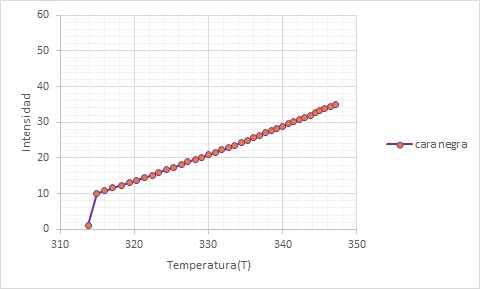
\includegraphics[width=0.7\textwidth]{negra.jpg}  
\caption{Intensidad vs Temperatura}
\label{uno}
\end{center}
\end{figure}


\begin{figure}[H]
\begin{center}
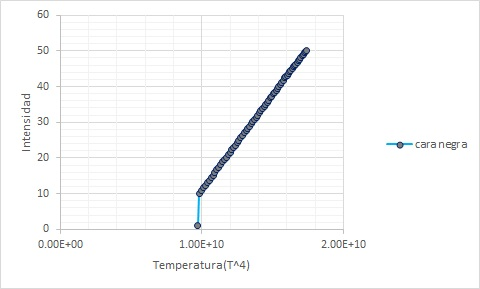
\includegraphics[width=0.7\textwidth]{negrat4.jpg}  
\caption{Intensidad vs $T^4$}
\label{2}
\end{center}
\end{figure}


\begin{figure}[H]
\begin{center}
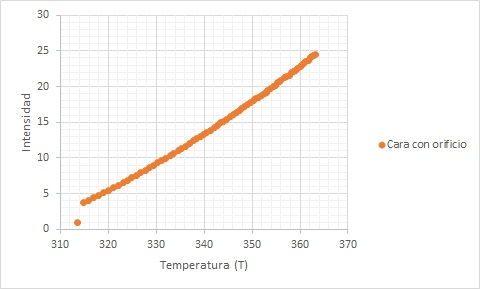
\includegraphics[width=0.7\textwidth]{orificio.jpg}  
\caption{Intensidad vs Temperatura}
\label{uno}
\end{center}
\end{figure}


\begin{figure}[H]
\begin{center}
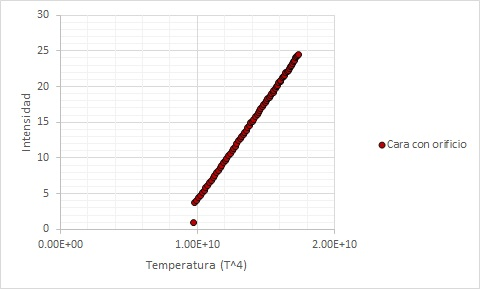
\includegraphics[width=0.7\textwidth]{orificiot4.jpg}  
\caption{Intensidad vs $T^4$}
\label{4}
\end{center}
\end{figure}
Para la segunda actividad se utilizó la ecuación (1), la ley de Ohm $R=VI$ y los datos de corriente y voltaje obtenidos por DataStudio para encontrar la temperatura del filamento.
Usando un voltaje de $6.17 V$ y una corriente de $1 A$
$R=6.17 \Omega$ una temperatura ambiente o referencia de $27 ^0C$ y una resistencia de referencia de $0.84\Omega$

$$T= 1436.05 ^0C$$
%===================================================================================================
\section{Discusión}
Se puede observar de las figuras \ref{2} y \ref{4} que la intensidad de radiación tiene una relación con la $T^4$, como se se encuentra en los libros de texto. Ademas se ve que el color y la forma de la superficie de la cara alteran la radiación que se detecta. Lo que se vio fue que la intensidad de la cara negra era casi el doble que la intensidad obtenida con la cara con orificio.

Para la segunda actividad se pensó que la intensidad del filamento no cambiaría tanto dependiendo del voltaje pero esto fue lo contrario a lo observado en el experimento, dado que al elevar el voltaje la intensidad de color en el filamento era cada vez mayor.
%===================================================================================================
\section{Conclusiones}
Se pudo concluir que en la primera actividad la cara que absorbe más energía es la pintada de color negro dado que la intensidad obtenida con ella fue más grande.

Para la segunda actividad se puede concluir que el voltaje tiene una relación directa con la temperatura del filamento esto debido a que según la ley de Ohm el voltaje es directamente proporcional a la resistencia y siguiendo la ecuación (1) la temperatura depende totalmente de la resistencia.

Además sabemos que la temperatura es inversamente proporcional al coeficiente de resistividad y como este era muy pequeño obtuvimos una temperatura muy elevada.

%================================================================================================	


\begin{thebibliography}{6}

\bibitem{a}
Universidad de Sevilla(s.f.) \textit{Trabajo en termodinámica} Recuperado de:
\url{http://laplace.us.es/wiki/index.php/Trabajo_en_termodin\%C3\%A1mica_(GIE)}

\bibitem{acu}
Acuña, H. (2015). \textit{Manual de Guías de Experiencias en el Laboratorio de Termodinámica Clásica}.

\bibitem{W}
Zemansky, M., Dittman, R.(1990) \textit{Calor y Termodinámica}


\end{thebibliography}
%================================================================================================


\end{document}
